\documentclass[11pt, a4paper]{article}
\usepackage[utf8]{inputenc}
\usepackage[margin=1in]{geometry} %Sets proper 1-inch margins. 
\usepackage{amsmath} %Only load this if you are using math/equations.
\usepackage{graphicx} %Only need to call this if inserting images.
%\usepackage{caption} %Only need to call this if inserting captions.
\usepackage{float} %Allows the use of the [H] specifier. 
%\graphicspath{{C:/Users/jonah/Pictures/}} %Sets the working directory for images.
\usepackage[colorlinks,citecolor=blue,linkcolor=blue,urlcolor=blue]{hyperref} %Allows for the embedding of urls. 
\usepackage{setspace}
\usepackage{blindtext}

\pagenumbering{arabic}

%\usepackage{fontspec} %%in order for this font stuff to work, you must compile using xelatex+makeindex+bibtex (or at minimum xelatex)
%\setmainfont[Mapping=tex-text-ms]{Essays1743}

\usepackage{fancyhdr}

\pagestyle{fancy}
\fancyhf{}
\rhead{Greenough \& Edmundson \\ 2023}
\lhead{\thepage}

\newcommand{\comment}[1]{}

\usepackage{Sweave}
\begin{document}
\Sconcordance{concordance:exploratory_analysis.tex:exploratory_analysis.Rnw:%
1 26 1 1 0 21 1 1 6 3 0 1 5 18 0 1 3 2 1 1 21 4 0 1 2 2 1 1 3 3 0 1 4 3 %
0 1 4 3 0 1 4 3 0 1 4 4 0 1 2 5 1 1 3 3 0 1 3 1 0 1 2 2 1 1 26 1 2 9 1 %
1 13 11 0 1 2 21 1 1 5 23 0 1 3 1 0 1 2 6 1 1 2 3 0 1 1 6 0 1 4 10 1 1 %
2 3 0 1 3 5 0 1 2 8 1 1 3 29 0 1 2 8 1 1 5 11 0 1 2 9 1 1 5 7 0 1 1 7 0 %
1 2 7 1}


\begin{center}
\LARGE{DATA583 Exploratory Analysis}
\par
\vspace{1.0pc}
\par
\large{Madison Greenough \& Jonah Edmundson}
\end{center}


\vspace{0.917 pc} %Creates a paragraph line break. 

%\pagebreak

%\tableofcontents

\section{Summary Statistics}

There are 10 variables for each listing, including the price of the listing (integer in \$USD), number of bedrooms (numeric, int), number of bathrooms (numeric), square feet (numeric), address (string), flag of whether it is new or not (binary 0 or 1), the listing company name (string), latitude (numeric), longitude (numeric), and distance to Central Park (numeric). Below we a summary of all numeric variables. Given is the minimum, quartiles, maximum, and median. This gives a great background and summary of the major variables here, especially our response variable, Price. Note that since the newflag variable is binary, this summary shows simply the count of which are new (True) and which are not (False).

\begin{Schunk}
\begin{Soutput}
Number of rows in dataset: 822
\end{Soutput}
\begin{Soutput}
     price               bed              bath             feet         
 Min.   :  132500   Min.   : 0.000   Min.   : 1.000   Min.   :     1.0  
 1st Qu.:  561250   1st Qu.: 1.000   1st Qu.: 1.000   1st Qu.:   863.8  
 Median :  875000   Median : 2.000   Median : 2.000   Median :  1285.0  
 Mean   : 1606935   Mean   : 2.912   Mean   : 2.399   Mean   :  3087.6  
 3rd Qu.: 1584750   3rd Qu.: 4.000   3rd Qu.: 3.000   3rd Qu.:  2368.5  
 Max.   :46395000   Max.   :24.000   Max.   :16.000   Max.   :325000.0  
                    NA's   :15       NA's   :27       NA's   :248       
    latitude       longitude         distance       
 Min.   :40.51   Min.   :-77.77   Min.   :  0.2015  
 1st Qu.:40.65   1st Qu.:-73.99   1st Qu.:  4.2443  
 Median :40.74   Median :-73.96   Median : 11.0958  
 Mean   :40.73   Mean   :-73.95   Mean   : 13.1292  
 3rd Qu.:40.77   3rd Qu.:-73.91   3rd Qu.: 18.2800  
 Max.   :42.64   Max.   :-73.59   Max.   :346.8985  
 NA's   :206     NA's   :206      NA's   :206       
\end{Soutput}
\end{Schunk}

Testing for outliers was done by calculating the z-score for each variable individually, within each row. Any z-score value greater than 3 was removed. 

\begin{Schunk}
\begin{Soutput}
Number of rows after outliers removed: 787
\end{Soutput}
\end{Schunk}

To confirm that the outliers were removed justly, a comparison was done between the outlier values and the dataset after the outliers were removed. Below, we see the difference between the two datasets in the median price, feet, bed, and bath. These are our primary numeric variables in the dataset. See below that there is a significant (greater) difference in the outlier median values compared to the new filtered dataset without them. This justifies the removal of these 35 instances.

\begin{Schunk}
\begin{Soutput}
Comparing outlier houses to non-outlier houses:
\end{Soutput}
\begin{Soutput}
  Median.price median.outlier.price
1       850000              3150000
\end{Soutput}
\begin{Soutput}
  Median.feet median.outlier.feet
1      1228.5              4679.5
\end{Soutput}
\begin{Soutput}
  Median.bed median.outlier.bed
1          2                  8
\end{Soutput}
\begin{Soutput}
  Median.bath median.outlier.bath
1           2                   6
\end{Soutput}
\end{Schunk}

Note that the outliers were removed based on individual values. A multivariate outlier detection would be superior, as it would take covariance into account when considering the distance between variables within rows, rather than each variables individually. A technique to measure this could be Mahalanobis distance, however, as some rows are missing various individual values, this leads to an NA value for the entire row, thus resulting in the current outlier approach looking at variables separately, without covariance considered. Moving forward, this could be a method to improve upon.
\par

Next, the pairs plot below shows not only the correlation between variables, but also the distribution of each. It seems as though that even with the outliers removed, the distribution of the response variable (price) is heavily right-skewed. This will result in the need for a GLM rather than a SLR in order to model price correctly. The distance measurement plots appear to have a `V' shape to them. This is a unique pattern to note. One prediction as to why this is happening, is that it could model the layout of the city, where the distinct V line lies around the water which is the boundary of the land of New York City, which is the location of this dataset.

\begin{Schunk}
\begin{Soutput}
Pairs plot for data with no outliers:
\end{Soutput}
\end{Schunk}
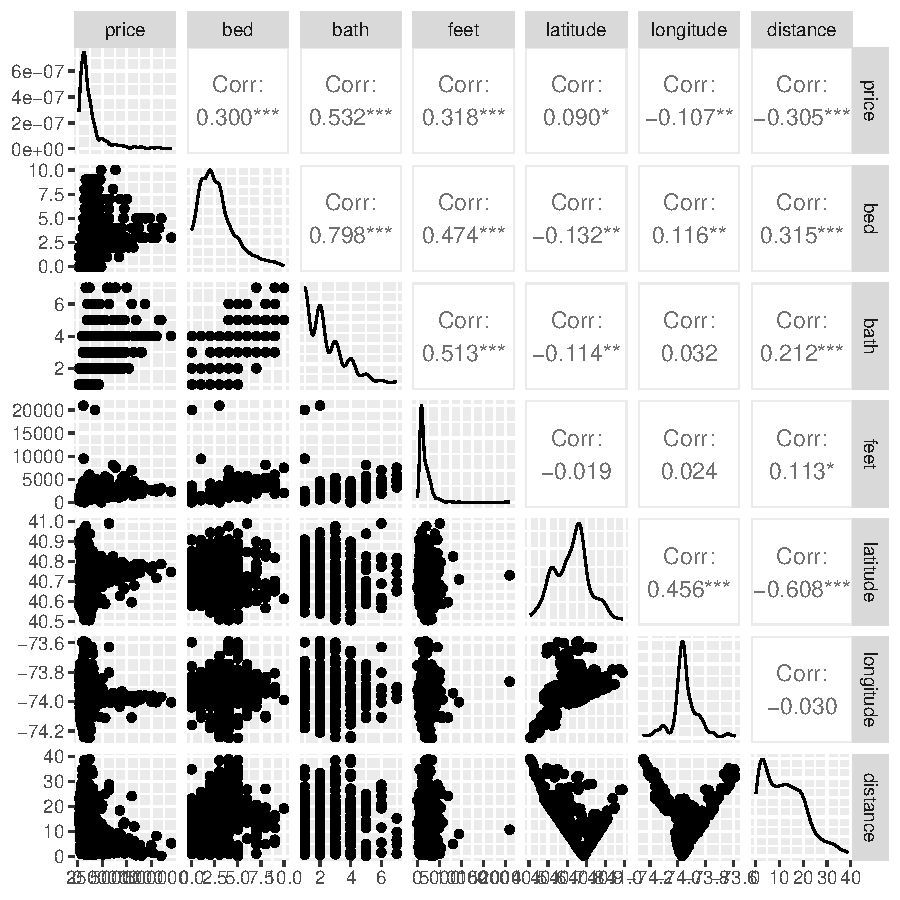
\includegraphics{exploratory_analysis-004}

Below, see a visualization of the missing data. 

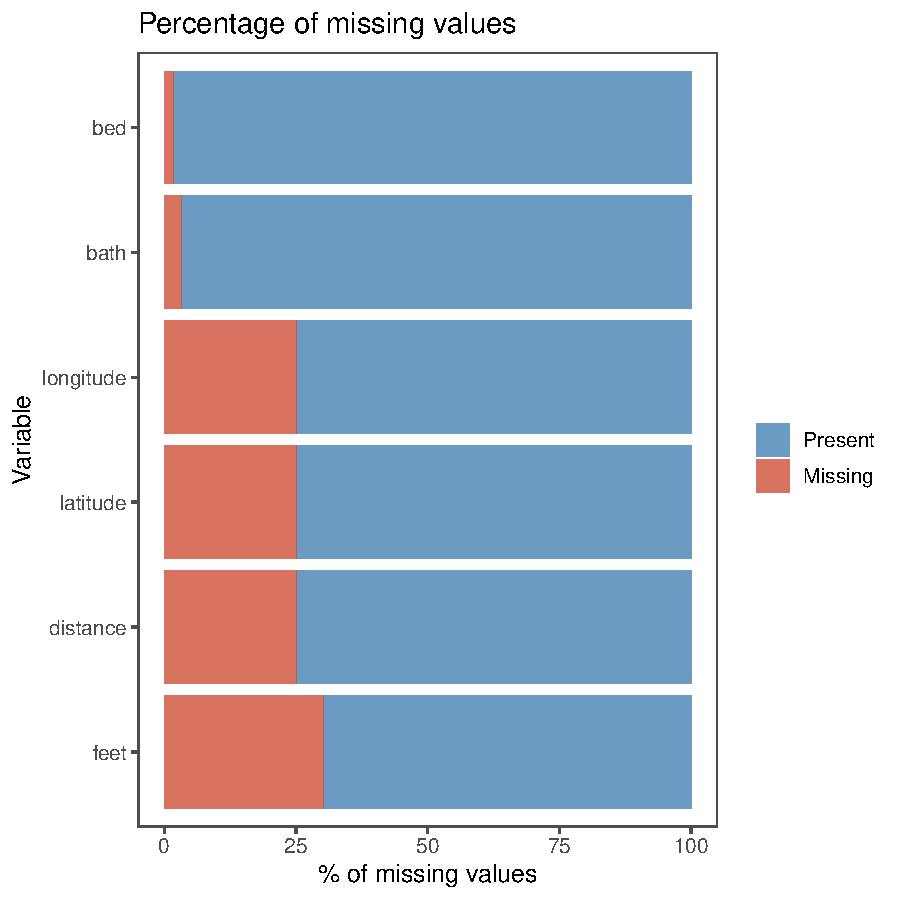
\includegraphics{exploratory_analysis-005}

There are missing data points throughout the dataset, given the nature of how the data
comes from many different listing agencies which have different protocols. Very few, <5\% of listings were missing bedroom or bathroom details. Approximately 25\% of the dataset has missing latitude or longitude values, which in turn results in 25\% of distance measures, as it is calculated from those values. Also, square footage is missing in approximately 30-35\% of the dataset.

\pagebreak

\section{Application of Techniques}

To begin, a Principal Component Analysis was done on the variables.

\begin{Schunk}
\begin{Soutput}
            PC1   PC2 PC3
bed          NA -0.68  NA
bath         NA -0.69  NA
feet         NA    NA  -1
latitude  -0.51    NA  NA
longitude  0.51    NA  NA
distance  -0.65    NA  NA
\end{Soutput}
\end{Schunk}
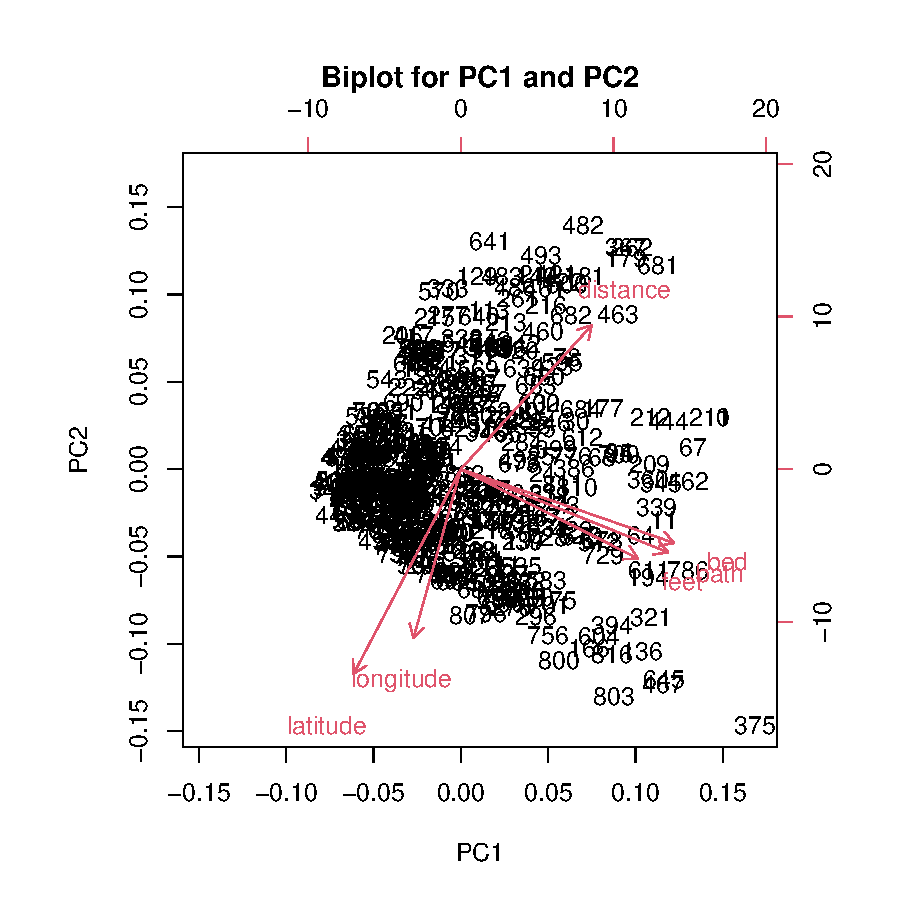
\includegraphics{exploratory_analysis-006}

It seems as though PC1 is measuring `location', PC2 indicates the housing `features' (number of bed and bath only), and PC3 measures the `size' of the property, indicated by `feet', as in square feet. 
\par
The PCA was run on the entire dataframe, including the outliers. When outliers are included, the results of PCA are intuitive. However, when outliers are removed, the results change drastically, and are no longer intuitive. This is a question leading into the report further to understand this further. 
\par
Also note that the plot of the PCA below has the outliers removed, to help with scaling and the visualization.
\par
To continue applying various learned techniques, see the prelimiary analysis section for different model fittings and preliminary assessment of scientific questions.

Notice in the plot the `V' shape looks similar to the plotting from the distance measurement in the pairs plot from above, but it is rotated now. This is an interesting shape, and we see that distance is in the exact opposite direction of latitude and longitude. Also, bed, bath, and feet are in the same general area, which makes sense, as they are similar measurements in the sense that the larger they are, the price would be expected to go up as well.

\section{Scientific Questions}

The goal of this analysis is to provide a model to predict housing prices in New York City. Price is the response variable, and the remaining variables are potential explanatory variables. A scientific question to answer, is, can the remaining variables be used to predict prices of listings in New York City? Another question, more specifically, which variables are more significant when predicting price, and can distance from Central Park be a useful measure to predict price? Potential future uses for the model is to apply it to different locations. 
\par
\par
Clustering is a potential modelling method that could be used for this dataset. The plan is to map various combinations of latitude and longitude onto different neighbourhoods in New York City to identify if there are differences in the clusters, or neighbourhoods.

\section{Statistical Analysis Techniques and Preliminary Results}

A linear model was run with price as the predictor, then bed, bath, feet, and distance as the explanatory variables. Below is the linear model summary output, as well as the residual plot, qqplot, and more.

\begin{Schunk}
\begin{Soutput}
Call:
lm(formula = price ~ bed + bath + feet + distance, data = no_outliers)

Residuals:
     Min       1Q   Median       3Q      Max 
-3797955  -557376   -92585   374529  6303568 

Coefficients:
              Estimate Std. Error t value Pr(>|t|)    
(Intercept)  800982.54  118379.12   6.766 4.58e-11 ***
bed         -155867.64   42784.06  -3.643 0.000304 ***
bath         722898.56   61568.61  11.741  < 2e-16 ***
feet            133.49      41.57   3.211 0.001427 ** 
distance     -65228.95    5938.99 -10.983  < 2e-16 ***
---
Signif. codes:  0 '***' 0.001 '**' 0.01 '*' 0.05 '.' 0.1 ' ' 1

Residual standard error: 1040000 on 410 degrees of freedom
  (372 observations deleted due to missingness)
Multiple R-squared:  0.4929,	Adjusted R-squared:  0.488 
F-statistic: 99.64 on 4 and 410 DF,  p-value: < 2.2e-16
\end{Soutput}
\end{Schunk}
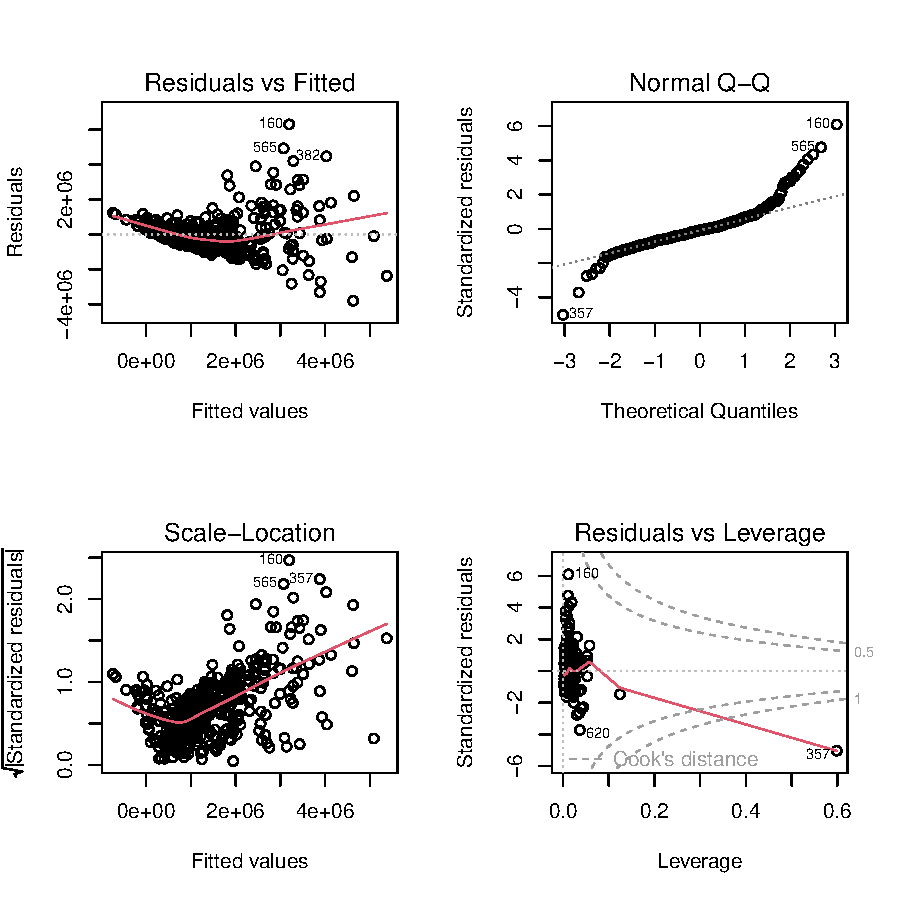
\includegraphics{exploratory_analysis-007}

Note that, at first glance, all variables appear significant, and the overall model p-value is also very significant. The adjusted R-squared value is moderate, at 0.49 approximately, meaning about half of the variation is explained by the model. If we look at the residual standard error, it is significantly greater than the degrees of freedom. This calculation was performed on the dataset after the outliers were removed. When performed on the original dataset, the p-values differed greatly. The results were also varied based on which variables were included.
\par
The residual plots show that there appears to be a lot of heteroskedasticity within the residuals. This implies that a linear model is likely not the best approach.
\par
There is one main outlier in the Cook's distance plot. Below is the point information specifically.

\begin{Schunk}
\begin{Soutput}
Point 375 and 27 are significant outliers in Cook's Distance:
\end{Soutput}
\begin{Soutput}
     price bed bath  feet                              address new_flag
357 569000   3    2 20930 9740 62nd Dr #7J,Rego Park, NY 11374     True
                                 company latitude longitude distance
357 EAST COAST REALTY PARTNERS BY ZARINA 40.73093 -73.86458 10.62326
\end{Soutput}
\end{Schunk}

It seems as though this point is unusually influential because it is very cheap (low price value) given the large size in features (number of beds, baths, and square footage size). This point was not removed by the outlier algorithm because each variable was only considered in isolation, and covariance was not accounted for. As mentioned above, in the final report, it may be beneficial to use Mahalanobis distance to detect outliers, as this algorithm \textit{does} take covariance into account, and would remove these types of points. 


\pagebreak
Modelling GLMs


\par
From the pairs plot above, it appears that the inverse Gaussian distribution would be the best fit when attempting to model price. However, there is a problem:

\begin{Schunk}
\begin{Soutput}
glm(price~bed+bath+feet+distance, data=no_outliers, family = inverse.gaussian)
\end{Soutput}
\begin{Soutput}
Error: no valid set of coefficients has been found: please supply starting values
In addition: Warning message:
In sqrt(eta) : NaNs produced
\end{Soutput}
\end{Schunk}

This is the same problem encountered in this paper:
\par
\url{https://link.springer.com/chapter/10.1007/978-1-4419-0118-7\_11}
\par
Given this error, it may be worth looking into potential solutions, or alternate ways to use a right-skewed distribution, as the dataset appears to follow.
\par
GLM can only be fitted on a few select model types with this dataset, and they appear to al have a very large deviance value relative to the degrees of freedom. This indicates that it is a poor fitting model. See below for the summary of a Gaussian fitted GLM.

\begin{Schunk}
\begin{Soutput}
Call:
glm(formula = price ~ bed + bath + feet + distance, family = gaussian, 
    data = no_outliers)

Deviance Residuals: 
     Min        1Q    Median        3Q       Max  
-3797955   -557376    -92585    374529   6303568  

Coefficients:
              Estimate Std. Error t value Pr(>|t|)    
(Intercept)  800982.54  118379.12   6.766 4.58e-11 ***
bed         -155867.64   42784.06  -3.643 0.000304 ***
bath         722898.56   61568.61  11.741  < 2e-16 ***
feet            133.49      41.57   3.211 0.001427 ** 
distance     -65228.95    5938.99 -10.983  < 2e-16 ***
---
Signif. codes:  0 '***' 0.001 '**' 0.01 '*' 0.05 '.' 0.1 ' ' 1

(Dispersion parameter for gaussian family taken to be 1.081214e+12)

    Null deviance: 8.7422e+14  on 414  degrees of freedom
Residual deviance: 4.4330e+14  on 410  degrees of freedom
  (372 observations deleted due to missingness)
AIC: 12684

Number of Fisher Scoring iterations: 2
\end{Soutput}
\end{Schunk}

Again, the deviance strays significantly from the degrees of freedom, indicating a poor model fit. Due to the odd distributions of each of the predictors as well as the response variable, parametric regression may prove difficult. 


\pagebreak
Modelling with Random Forests
\par
Next, Random Forests will be used to attempt to model this dataset.

\begin{Schunk}
\begin{Soutput}
Call:
 randomForest(formula = price ~ bed + bath + feet + distance,      data = no_outliers, na.action = na.roughfix) 
               Type of random forest: regression
                     Number of trees: 500
No. of variables tried at each split: 1

          Mean of squared residuals: 7.02956e+11
                    % Var explained: 64.03
\end{Soutput}
\end{Schunk}

Note that it was needed to set \texttt{na.action = na.roughfix} due to missing values (thanks to \href{https://stackoverflow.com/questions/8370455/how-to-use-random-forests-in-r-with-missing-values}{this} SO post). 

While a fair amount of the variation is explained by the model, the squared residuals are extremely high. This is concerning, and indicates that this may not be the correct method for this dataset. 

\pagebreak
Modelling with Boosting
\par
Next, boosting will be used to attempt to model this dataset.

\begin{Schunk}
\begin{Soutput}
gbm(formula = price ~ bed + bath + feet + distance, distribution = "tdist", 
    data = no_outliers, n.trees = 5000, interaction.depth = 1)
A gradient boosted model with tdist loss function.
5000 iterations were performed.
There were 4 predictors of which 4 had non-zero influence.
\end{Soutput}
\begin{Soutput}
              var   rel.inf
distance distance 40.514605
bed           bed 35.640760
feet         feet 19.995500
bath         bath  3.849136
\end{Soutput}
\end{Schunk}

Above, the summary output for the boosting model is shown. All four predictors had an influence, which is positive, and distance appeared to be the strongest. Square footage was close behind, but bed and bath were significantly less influential. It is interesting to note that distance, the variable created from the latitude and longitude measures, was the most influential. This is a variable that is not given in the scraped data, and it is not typically available to buyers or sellers when looking at a home. It was created to represent the distance from Central Park, a common attraction and central part of the city. This is an interesting outcome, as it shows that it may be a useful tool in predicting price for this model, but if this model were to be used in a different location other than New York City, it would not be transferable.

\vspace{2pc}

Moving forward, the target model for this dataset is clustering, so various clustering algorithms will be used to attempt to model this dataset. Hierarchical clustering, k-means clustering, as well as mixture models, are some methods to be explored, to name a few. Clustering will likely fit this dataset the best because, given the nature of the distance variable, it would be helpful to cluster based on neighbourhoods, as well as different housing features within the neighbourhood. For example, the Upper East Side of New York, which is known to be an elite neighbourhood, could be identified by the clustering algorithm, and then further cluster within the neighbourhood to group based on the size of the listing (including beds, baths, and square footage). It would be useful to have these levels clustered to help with predicting prices, both from a buyer and seller perspective. This could help homeowners when determining a list price for a home, and it could also help buyers to determine their budget based on their given variable criteria, as well as to evaluate given prices of listings to determine if they are reasonable or not. If the clustering algorithm succeeds with this dataset, it could mean that many different audiences will have access to a tool to help them in their home buying and selling journey. It could also be used as a tool sold to listing companies to help them with home evaluations and listings.

\end{document}
